\documentclass[a4paper, titlepage]{article}
\usepackage[round, sort, numbers]{natbib}
\usepackage[utf8]{inputenc}
\usepackage{amsfonts, amsmath, amssymb, amsthm}
\usepackage{color}
\usepackage{framed}
\usepackage{listings}
\usepackage{mathtools}
\usepackage{paralist}
\usepackage{parskip}
\usepackage{subfig}
\usepackage{tikz}
\usepackage{titlesec}

\numberwithin{figure}{section}
\numberwithin{table}{section}

\usetikzlibrary{arrows, automata, backgrounds, petri, positioning}
\tikzstyle{place}=[circle, draw=blue!50, fill=blue!20, thick]
\tikzstyle{transition}=[rectangle, draw=black!50, fill=black!20, thick]

% define new commands for sets and tuple
\newcommand{\setof}[1]{\ensuremath{\left \{ #1 \right \}}}
\newcommand{\tuple}[1]{\ensuremath{\left \langle #1 \right \rangle }}
\newcommand{\card}[1]{\ensuremath{\left \vert #1 \right \vert }}

\makeatletter
\newcommand\deadline[1]{\def\@deadline{#1}}
\newcommand\objective[1]{\def\@objective{#1}}
\newcommand{\makecustomtitle}{%
	\begin{center}
		\huge\@title \\
		[1ex]\small Dimitri Racordon, le \@date
	\end{center}
	\begin{framed}\@deadline\end{framed}
	\begin{framed}\@objective\end{framed}
}
\makeatother

\begin{document}

  \title{Outils formels de Modélisation \\ 1\textsuperscript{er} Travail personnel}
  \author{Dimitri Racordon}
  \date{23.09.15}

	\deadline{
		\textbf{Date de rendu}: Jeudi 12.10.17 à 23h55 \\

		Comme leur nom l'indique, ces travaux sont \emph{personnels}.
		La copie est strictement interdite, et toutes similitudes entre deux rendus
		seront santionnées par la note de 0.
		Tout dépassement de la date et heure de rendu sera lourdement pénalisée.
		Date et heure de rendu sont toujours données en heure locale de Genève.
		Tout commit sur votre dépôt publié après la date de rendu sera ignoré.

    Seule la branche \texttt{master} de votre dépôt sera prise en compte
    lors de la correction.

		Votre code doit être compilable en Swift 4.0, avec un compilateur officiel.
		La note the 1 vous sera attribuée si votre code ne peut être compilé.
	}

	\objective{
    Dans ce TP, vous allez utiliser le formalisme des réseaux de Petri
    afin de corriger un comportement indésirable dans un système concurrent et non déterministe.

		Prenez le temps d'étudier le système afin de bien comprendre le problème à corriger,
    ainsi que ses implications.
	}

	\makecustomtitle

  \section{Spécification}
		Considérez le modèle d'un gestionnaire de tâches décrit par la spécification suivante:
		\begin{enumerate}
		  \item Lorsqu'une tâche arrive, elle est placée dans ensemble des tâches à exécuter.
		  \item Lorsqu'un nouveau processus est prêt à exécuter une tâche,
            il est placé dans un autre ensemble.
		  \item Lorsque que c'est possible,
            le gestionnaire sélectionne une tâche et un processus pour l'exécuter.
				    Le processus sélectionné est alors retiré de l'ensemble des processus disponibles.
		  \item Si la tâche réussit, elle est retirée de l'ensemble des tâches à exécuter
            et le processus est détruit.
		  \item Si la tâche échoue, elle reste dans l'ensembles de tâches à exécuter
            et le processus est détruit.
		\end{enumerate}
		Une implémentation de cette spécification vous a été proposée en Fig. \ref{fig:task-pool}.
		Cependant lors des tests,
    il arrive occasionnellement qu'un processus ne puisse jamais être détruit,
    malgré qu'il ait fini d'exécuter sa tâche.
		Votre mission est de corriger ce problème.

		\begin{figure}[ht]
			\centering
			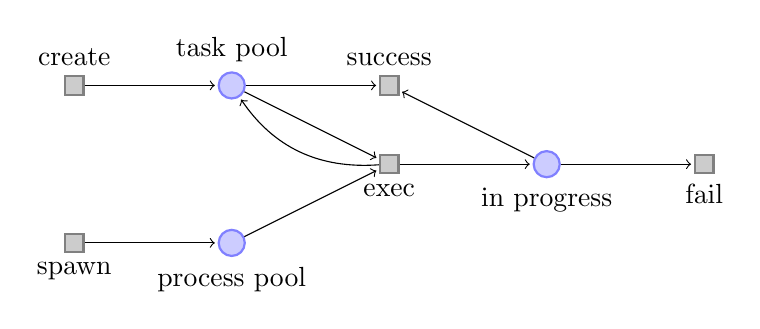
\begin{tikzpicture}[node distance=2cm]
				\node (placeholder) {};
				\node[place] (tp) [label=90:{task pool}] {};
				\node[place] (pp) [below of=tp, label=-90:{process pool}] {};
				\node[place] (ip) [right of=pp, xshift=2cm, yshift=1cm, label=-90:{in progress}] {};

				\node [transition] (t0) [left of=tp, label=90:{create}] {}
								edge [post] (tp);
				\node [transition] (t1) [left of=pp, label=-90:{spawn}] {}
								edge [post] (pp);
				\node [transition] (t2) [left of=ip, label=-90:{exec}] {}
								edge [pre] (tp) edge [pre] (pp)
								edge [post, bend left] (tp) edge [post] (ip);
				\node [transition] (t3) [right of=tp, label=90:{success}] {}
								edge [pre] (tp) edge [pre] (ip);
				\node [transition] (t4) [right of=ip, label=-90:{fail}] {}
								edge [pre] (ip);
			\end{tikzpicture}
			\caption{Gestionnaire de tâches}
			\label{fig:task-pool}
		\end{figure}

  \section{Mise en place du TP}
    Forkez le dépôt https://github.com/cui-unige/outils-formels-modelisation.
    Vous travaillerez sur votre propre version du dépôt,
    et effectuerez tous vos commit sur ce dépôt-ci.

    Le projet pour ce TP se trouve dans le répertoire \texttt{tp-01}.

	\section{Analyse du problème}
		A l'aide du réseau de la Fig. \ref{fig:task-pool},
    donnez un exemple d'exécution qui conduirait au problème décrit ci-dessus,
    sous la forme d'une suite d'exécution de la méthode \texttt{fire(from:)}
    sur les transitions appropriées.

  \section{Correction du problème}
		Modifiez le réseau de la Fig. \ref{fig:task-pool} afin de corriger le problème identifié,
    en modifiant la définition du P/T-net construit par la fonction \texttt{createCorrectTaskManager}.
		Vous pouvez ajouter autant de places et de transitions que vous le souhaitez,
    mais vous ne pouvez rien retirer du réseau existant.

		A l'aide de commentaires,
    expliquez en détail comment les modifications que vous avez apportées.

    Enfin, montrez que la séquence de transition que vous aurez définie pour illustrer le problème
    ne conduit plus à un marquage problématique.

\end{document}
